%!TEX root = index.tex
\chapter{Testing}

\red{TODO: intro}

\section{Comparison of scheduling algorithms on single runway}

This first test compares the performance of implemented scheduling algorithms. The scenario contains twelve flights with alternating weight class landing on one runway arriving in close succession. This scenario should be particularly demanding to be scheduled optimally because the alternation in weight classes make it sensitive to the order in which the slots are scheduled.

\begin{table}[h]
  \centering
\begin{tabular}{ | l | c | r | r | }
\hline
Flight id	& Weight class	& \red{Time of appearance on screen} & Runway arrival time	\\
\hline
01M	& MEDIUM	& 	& 42:30	\\
02J	& JUMBO		& 	& 42:29	\\
03J	& JUMBO		& 	& 44:15	\\
04M	& MEDIUM	& 	& 44:49	\\
05M	& MEDIUM	& 	& 46:30	\\
06J	& JUMBO		& 	& 46:29	\\
07J	& JUMBO		& 	& 48:15	\\
08M	& MEDIUM	& 	& 48:49	\\
09M	& MEDIUM	& 	& 50:30	\\
10J	& JUMBO		& 	& 50:29	\\
11J	& JUMBO		& 	& 52:15	\\
12M	& MEDIUM	& 	& 52:49	\\
\hline
\end{tabular}
  \caption{The configuration of the first test scenario}
  \label{tab:config1}
\end{table}

Table \ref{tab:config1} shows the configuration of the test scenario. For the \texttt{JUMBO} category the Airbus A380-800 was used and the \texttt{MEDIUM} category was represented by Boeing 737. Airplanes headed to the airport from two separate streams to prevent possible violation of separation in en-route sectors the planes fly from.

\begin{figure}[h]
    \centering
    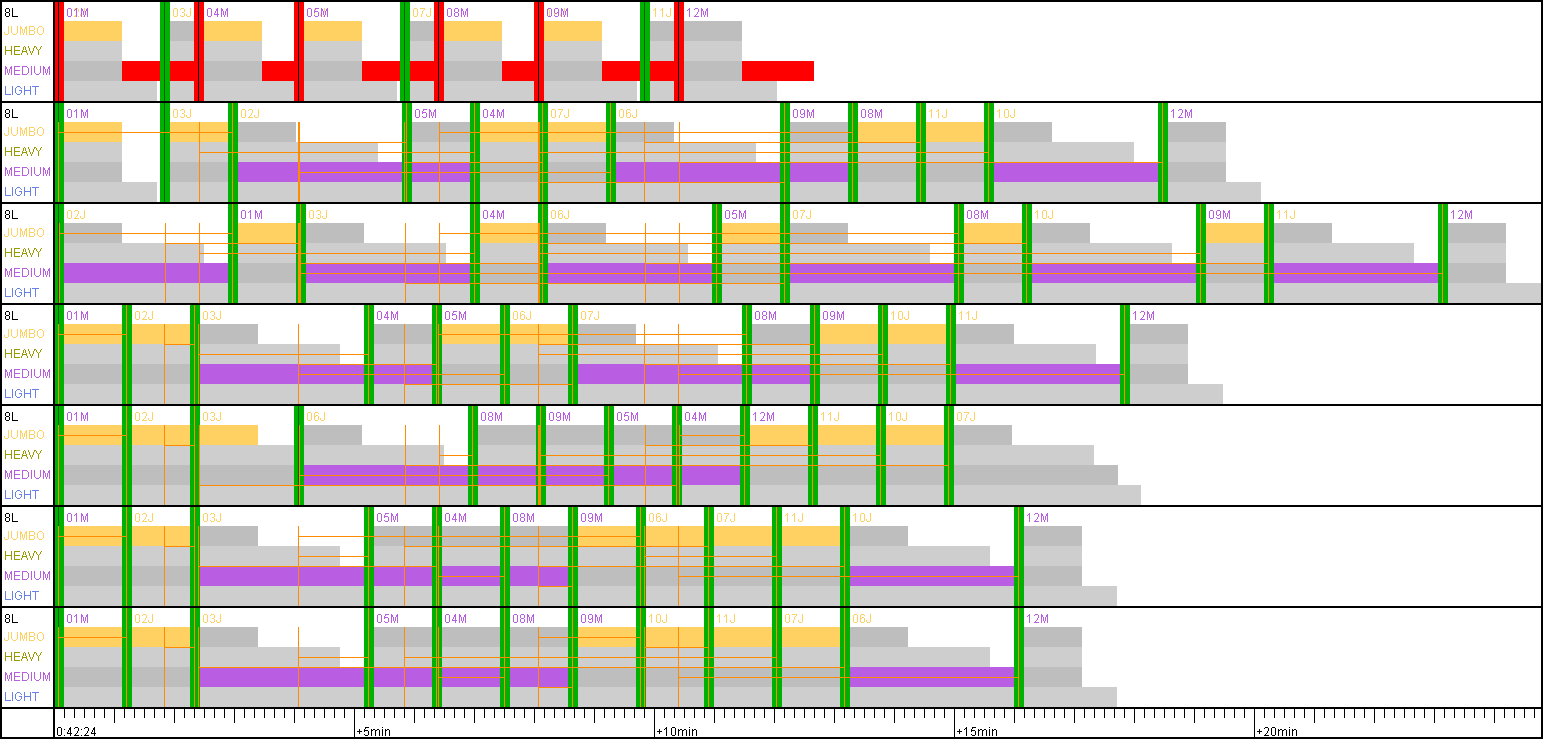
\includegraphics[width=\textwidth]{figures/1rwy-alternating.png}
    \caption{Result of planning with different algorithms on single runway}
    \label{fig:1rwy-alternating}
\end{figure}

The resulting plans are shown in Figure \ref{fig:1rwy-alternating}. The first row shows the result of {\em Algorithm~1} which places the slots in the exact time the arrival was estimated. It demonstrates how many collision would occur if no planning was present and serves as the lower bound on the total plan time.

The plans generated by {\em Algorithm~2} and {\em Algorithm~3} are identical in this case and are depicted in the second row. The slots are ordered in the same succession the corresponding aircraft appeared on the controller's screen. The reason the plans are identical is that the stream of arriving planes is very dense and there are no voids present between the aircraft the {\em Algorithm~3} would utilize to produce better schedule than {\em Algorithm~2}.

Third and fourth rows show the results of both versions of {\em Algorithm~4}. The third row contains the plan generated by the simple version of the algorithm, that keeps the order of aircraft's expected time of arrival. In this instance the algorithm produced the poorest result with the longest overall time as well as longest maximal and total delays. This is due to the specific configuration of the test scenario that alternates between weight classes. The second version doesn't rigorously keep the order of estimated arrival but tries to locally minimize the delays and therefore produces much better result.

The last three rows contain plans generated by the three versions of {\em Algorithm~5}. Each one shows optimal plan according to selected criterion. The one in the fifth row has the shortest total makespan. The plan in sixth row has the shortest maximal delay of a slot in the plan. And the last plan has minimal sum of delay of all slots. Note, that the last two plans are very similar and even have the same total length but the order of the slots determines whether the solution minimizes one or the other criterion.

\subsection{Makespan}

\begin{figure}[h]
    \centering
    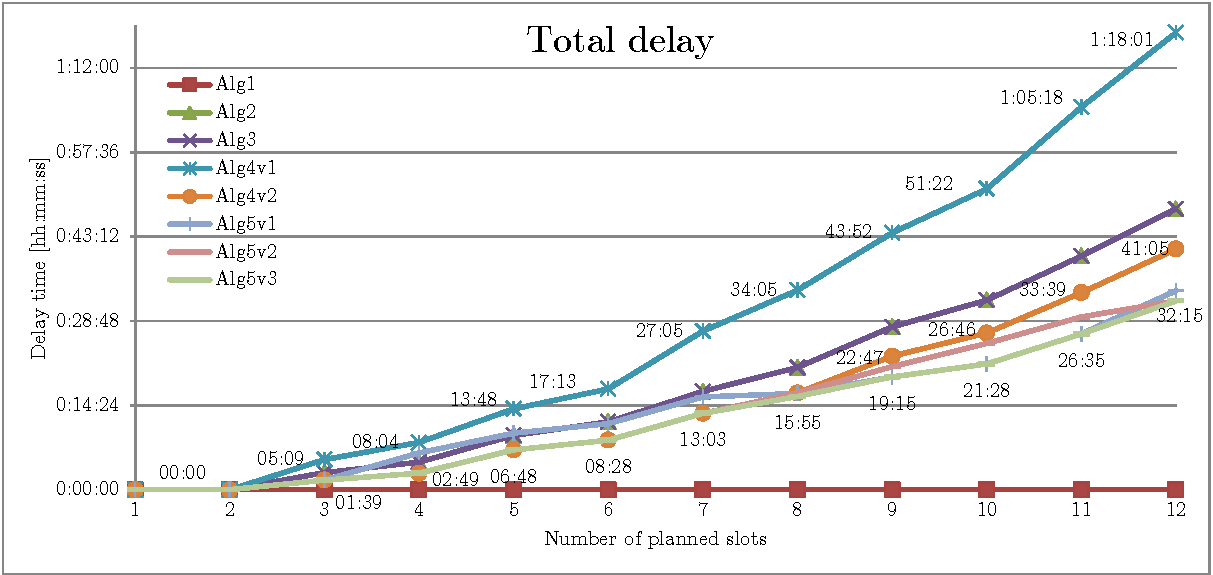
\includegraphics[width=\textwidth]{graphs/1rwy-alternating-total-delay.pdf}
    \caption{\red{Placeholder: update graph of makespan times}}
    \label{graph:1rwy-alternating-makespan}
\end{figure}

The obvious criterion by which the quality of a plan can be determined is the total duration of the schedule, also called makespan. The shorter the plan is, the better, because all the planes will in total land in the shortest possible time. In reality this criterion is problematic, because the flow of airplanes to the airport is infinite, only the density changes in time. But even so, this criterion can give a notion of the quality of immediate plan.

\red{TODO}

\subsection{Maximal delay}

\begin{figure}[h]
    \centering
    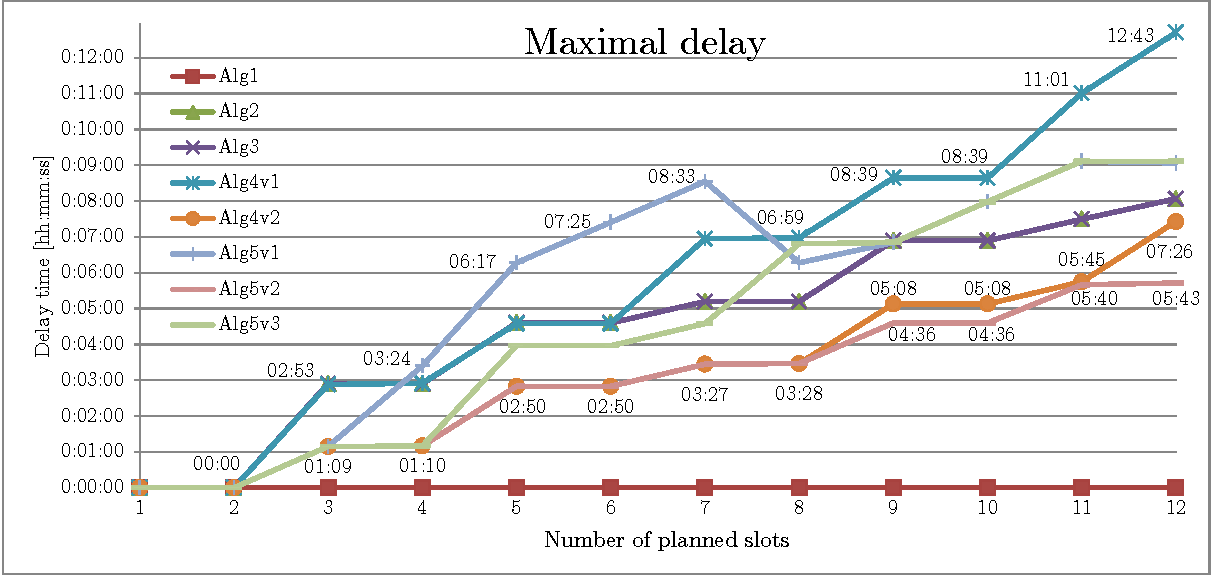
\includegraphics[width=\textwidth]{graphs/1rwy-alternating-maximal-delay.pdf}
    \caption{Graph of maximal delay for plans created with different algorithms on single runway}
    \label{graph:1rwy-alternating-maximal-delay}
\end{figure}

Another criterion that can describe the quality of a runway plan is the maximal delay among all slots. Obviously the smaller the delay is, the better the plan is. This criterion criterion can be used to prevent the situation in which one plane would give the priority to all others and would wait until its supply of fuel is depleted. The sum of all delays can be small, but the fact that the critical delay time for one aircraft was exceeded renders such plan potentially dangerous.

Graph \ref{graph:1rwy-alternating-maximal-delay} shows the development of values of this criterion during the planning. The optimal value for the final plan is 5 minutes and 43 seconds and is achieved by {\em Algorithm~5v2}. {\em Algorithm~4v1} has the poorest performance with the value of 12:43. {\em Algorithm~5v1} optimizes the total makespan and in order to do that it can delay some slots by a significant amount of time. This can lead to high maximal delay values as shown here for plans with 4 – 7 slots. {\em Algorithm~4v2} performs very well with its result at or very near the optimal value. For the final plan the maximal delay for this algorithm is 1 minute 43 second longer than the optimal value.

\subsection{Total delay}

\begin{figure}[h]
    \centering
    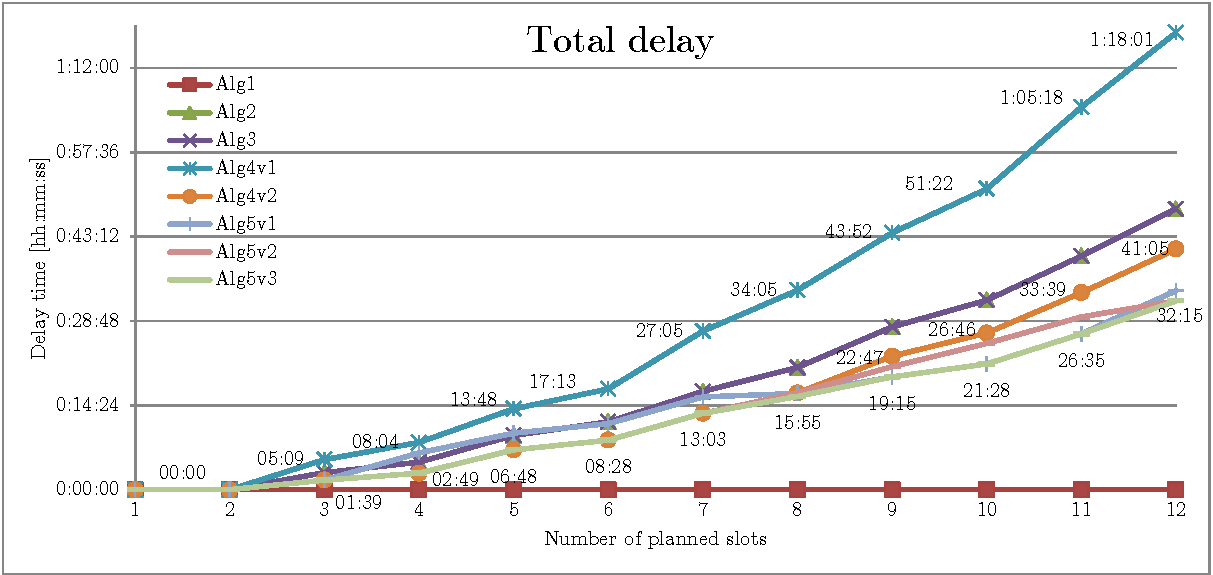
\includegraphics[width=\textwidth]{graphs/1rwy-alternating-total-delay.pdf}
    \caption{Graph of total delay for plans created with different algorithms on single runway}
    \label{graph:1rwy-alternating-total-delay}
\end{figure}

The sum of all slot delays is another way to measure runway plan's quality. It describes the total time wasted on waiting in the terminal area. It is also linked to the total amount of fuel burnt during the waiting. Both time and used amount of fuel affect the costs of the flight.

The total delay times in the progress of planning are shown in Graph \ref{graph:1rwy-alternating-total-delay}. The poorest results are again given by {\em Algorithm~4v1} with the total delay more than 2.4 times the optimum. The optimal result is produced by {\em Algorithm~5v3} (32:25 for final plan) with other two versions of the {\em Algorithm~5} very near. {\em Algorithm~4v2} performs well with the total delay at 41:05 which is less than 30\% more than the optimum. {\em Algorithm~2} and {\em Algorithm~3} still perform good and could produce usable results but are not as good as {\em Algorithm~4v2}.

\subsection{Replanned slots}

\begin{figure}[h]
    \centering
    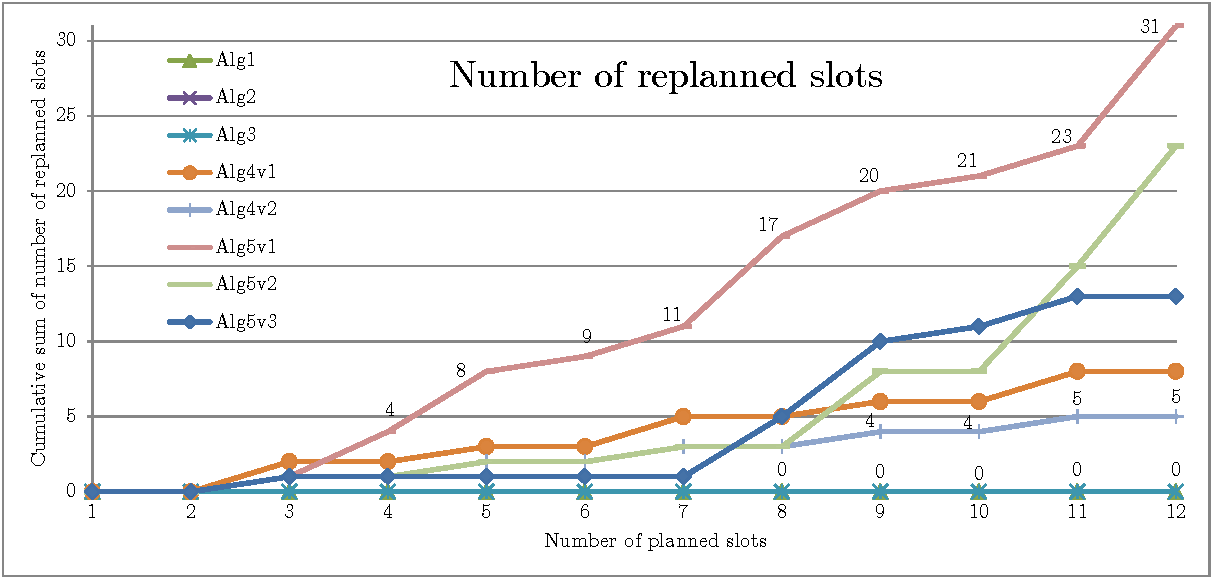
\includegraphics[width=\textwidth]{graphs/1rwy-alternating-replanned-slots.pdf}
    \caption{Graph of cumulative sum of replanned slots for plans created with different algorithms on single runway}
    \label{graph:1rwy-alternating-replanned-slots}
\end{figure}

The number of replanned slots shown in Graph \ref{graph:1rwy-alternating-replanned-slots} expresses how often the controller must interfere with the schedule of previously planned aircraft after a new one has been added to the plan. This criterion has a relation to the controllers workload, because he/she must contact each replanned aircraft and give the pilot updated instructions.

{\em Algorithm~1}, {\em Algorithm~2} and {\em Algorithm~3} place the new slots in a way that doesn't affect the previously planned and therefore don't cause the need to replan old slots. {\em Algorithm~4v2} with five replanned slots during the creation of final plan produces very good results according to the aforementioned criteria but is still undemanding of frequent replanning of old slots. All three versions of {\em Algorithm~5} have high numbers of replanned slots because the fat that they look for optimal solution causes them to change the plan significantly with each slot addition. This is especially true for {\em Algorithm~5v1} which minimizes the total makespan. Its 31 replanned slots during the creation of plan for 12 planes render it unusable for real world application.

\subsection{Conclusion}

\red{TODO}

\section{Real world flights on single runway}

\red{TODO}

%\section{Comparison To Real Air Traffic}
%\section{Flight Duration}
%\section{Fuel Consumption}
%\section{Controller Workload}
%\section{Airport/Runway capacity}